\subsection{Human Vision: Organization and Function}

We can now have a very brief look at human vision. We'll mostly focus on understanding our "photoreceptor" which is the retina and won't go into the processsing details of the visual cortex which, despite having been extensively documented since the work of Hubel and Wiesel in the 1960s \footnote{Hubel and Wiesel worked together at Harvard on visual processing in the cat. Their research, spanning over two or three decades, and for which they both received a Nobel Prize, remains some of the most influential works in Neuroscience to date.} is still an active domain of research because of its complexity. 

\subsubsection{General architecture of the visual system}

Some thing you should know about the architecture of the visual system: 
\begin{itemize}
    \item Retinal image inverted and reversed compared to the visual field
    \item The axons of retinal ganglion cells form the optic nerves.
    \item At the \textit{optic chiasm}, axons from the temporal halves of each retina continue into the optic tract of the same side. Axons from the nasal halves cross to the optic tracts on the opposite side. \textbf{So the myth that vision is systematically processed on the opposite side of the corresponding eye if false}. But the visual field is separated in two on each eye.  
    \item Most of the primary visual cortex (also called V1) is on the medial surface of the human brain (see figure). This is one of the key place where visual input is processed in the brain.
\end{itemize}

\begin{figure}[H]
    \centering
    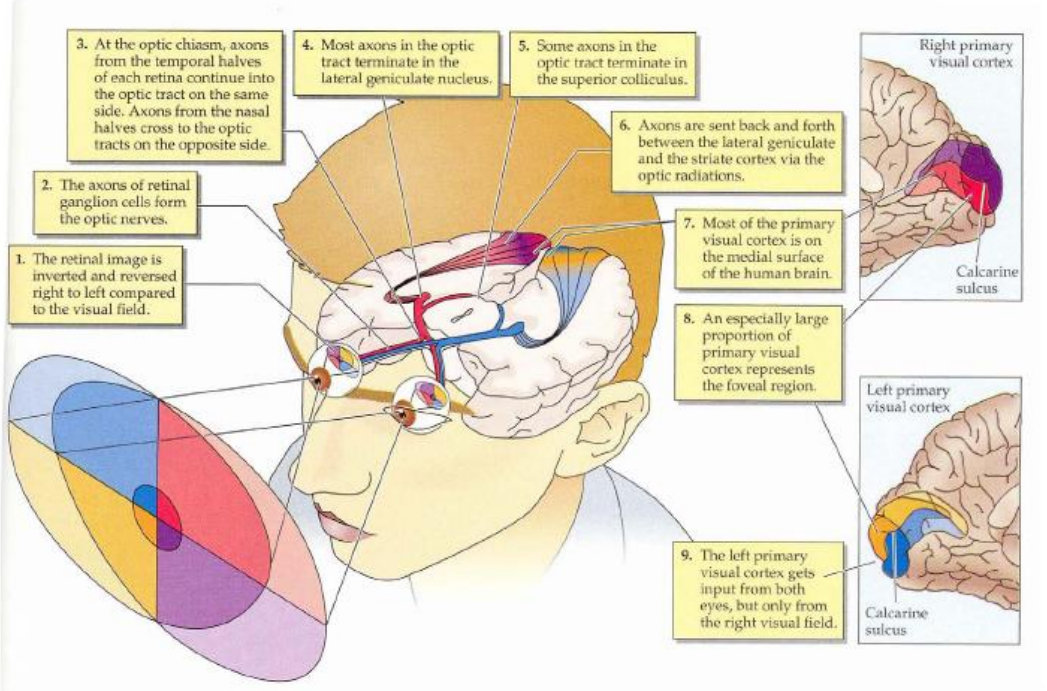
\includegraphics[width=0.9\linewidth]{../../Figures/Vision.PNG}
    \caption{Simplified structure of the Visual system. Adapted from somewhere on Google Image.}
    \label{Vision}
\end{figure}

\subsubsection{The human eye}

Not much to say, this is just about organizational things. The important bit it where the retina is, where interesting things happen.  

\begin{figure}[H]
    \centering
    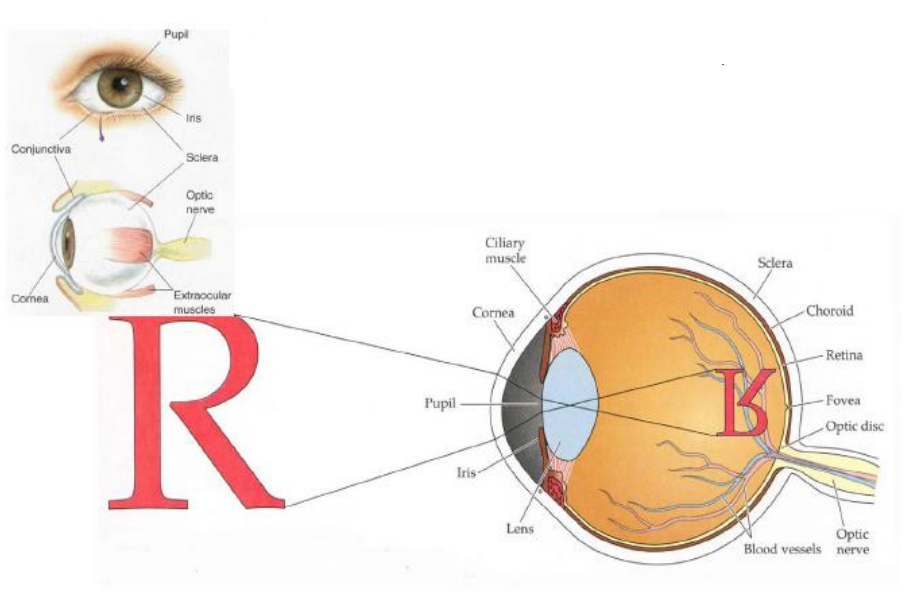
\includegraphics[width=0.9\linewidth]{../../Figures/Eye.PNG}
    \caption{Simplified structure of the eye. Adapted from somewhere on Google Image.}
    \label{fig:Eye}
\end{figure}

\subsubsection{The retina}

The retina is where the photoreceptors are located. The important processing happens first through the ganglion cells, followed by the bipolar cells and then reaching the cones and rods, which are the essential photoreceptors of the human eye. This is actually a bit counterintuitive: light \textbf{arrives first in the photoreceptors}, which are at the back of the retina. The photoreceptors will then transmit to the ganglion cells through the bipolar cells. Finally, the ganglion cells carry information from the retina to the brain. If you pay attention to the "wiring" in the figure, this should become clearer. 

\begin{figure}[H]
    \centering
    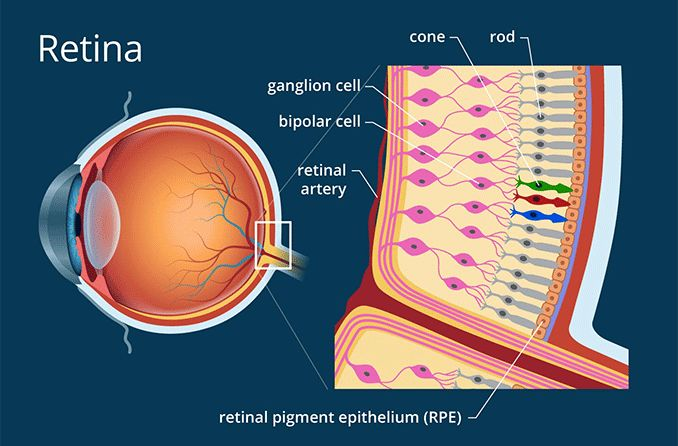
\includegraphics[width=0.7\linewidth]{../../Figures/Retina.png}
    \caption{Simplified structure of cells in the Retina. Light reaches first the photoreceptors (cones and rods), and transmit, through bipolar cells, to the ganglion cells which then transmit to the brain. Adapted from somewhere on Google Image.}
    \label{fig:Retina}
\end{figure}

\subsubsection{Human photoreceptors: Rods and Cones}

The most interesting part for NE1 is understanding the photoreceptors, their structure and organisation. There are two main types of photoreceptors in the retina: Rods and Cones. They are very particular types of neurons. Rods (~120 Millions) are very sensitive and are most useful in diminished light. They "saturate" at high illumination. Cones on the other end are much less numerous (~5 Millions) and are only sensitive to brighter light. There are also three different types of cones, each being specifically receptive to a range of wavelenght (colors). A summary of the distribution and optimal wavelenght for each type of photoreceptor is shown in figure \ref{fig:Cones_And_Rodes}.

\begin{figure}[H]
    \centering
    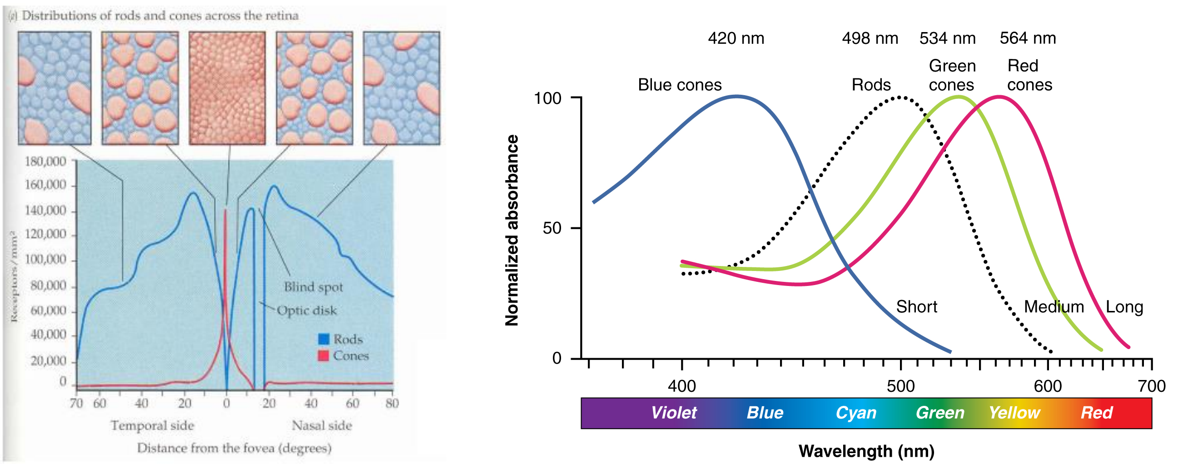
\includegraphics[width=0.9\linewidth]{../../Figures/Cones_And_Rodes.png}
    \caption{A) Distribution of Cones and Rods in the retina. B) Wavelenght absorbance of different types of photoreceptors of the retina. Adapted from somewhere on Google Image.}
    \label{fig:Cones_And_Rodes}
\end{figure}

We should also note that there are no rods but many cones in the \textit{fovea}: it is the region in our retina that provides the highest acuity of vision (see Cones peak region in figure \ref{fig:Cones_And_Rodes}). There are also no photoreceptors on the optic nerve (see figure \ref{fig:Eye}) which constitutes a \textit{blind spot}. 

\subsubsection{Photo receptor structure and function}


\begin{figure}[H]
    \centering
    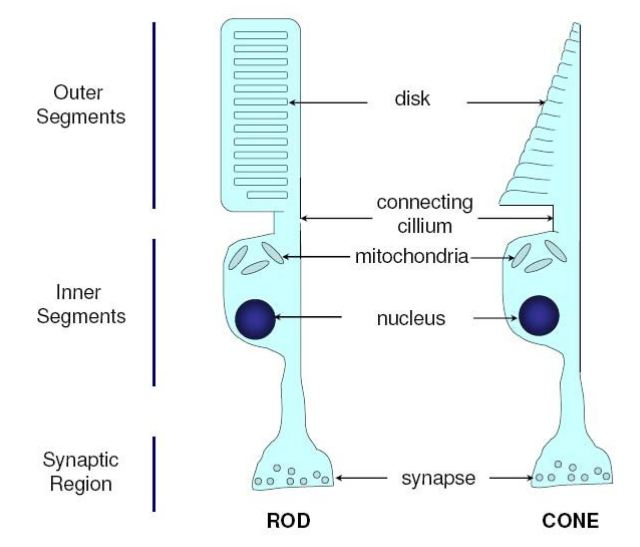
\includegraphics[width=0.55\linewidth]{../../Figures/Rods_And_Cones_Structure.jpg}
    \caption{Structure of Rods and Cones. Adapted from somewhere on Google Image.}
    \label{fig:Rods_And_Cones_Structure}
\end{figure}

As can be seen in figure \ref{fig:Rods_And_Cones_Structure}, rods and cones both possess "outer segment disks" which are filled with \textit{opsin}, a protein which absorbs photons as well as voltage gated Sodium (Na) channels. These proteins are actually slightly different in cones and rods: cones carry \textit{photopsin} whilst rods carry \textit{rhodopsin}. However, both actually function very similarly: photons being in contact with the opsin proteins are absorbed by the latter. This generates a biochemical cascade (including a decrease in \textit{Glutamate} release) leading to a hyperpolarization of the photoreceptor cell and eventually to triggering an \textit{action potential}. Bipolar cells subsequently respond to this hyperpolarization and things go on from there to the ganglion cells etc...
Figure \ref{fig:Cone_Rode_Response} shows the change in current after light trigger (at time 0) through the photoreceptors.  

\begin{figure}[H]
    \centering
    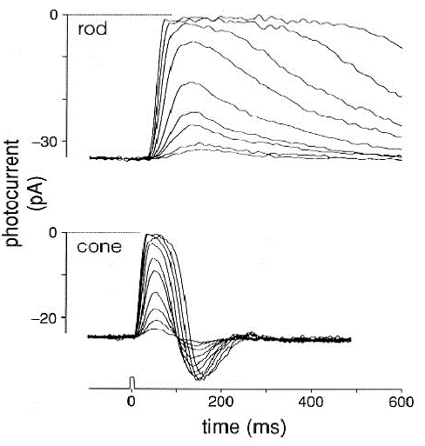
\includegraphics[width=0.5\linewidth]{../../Figures/Cone_Rod_Response.PNG}
    \caption{Cones and Rods response to light. Adapted from somewhere on Google Image.}
    \label{fig:Cone_Rode_Response}
\end{figure}

Let's give a summary of the key points about photoreceptors, because this is what should be remembered: 

\begin{itemize}
    \item Photoreceptor cells are depolarized in the dark
    \item Light hyperpolarizes the cell, with activates the next cell in the neural pathway: bipolar cells. 
    \item In the dark, levels of Glutamate are high and allow a \textit{steady} inward \textit{dark} current. This keeps the cell at a depolarization value of about -40 mV. 
\end{itemize}
